\documentclass{report}
\title{`cs229'---Notes}
\date{Started 1st October 2024}
\author{Malcolm}
\usepackage{amsmath} %import math
\usepackage{mathtools} %more math
\usepackage{amssymb} %for QED symbol
\usepackage{amsthm} %
\usepackage{bm} %bolding without changing font
\usepackage{graphicx} %import imaging
\graphicspath{{./images/}} %set imaging path
\newcommand*{\vertbar}{\rule[-1ex]{0.5pt}{2.5ex}} %matrix
\newcommand*{\horzbar}{\rule[.5ex]{2.5ex}{0.5pt}} %matrix
\begin{document}
\maketitle
\tableofcontents

\chapter{Supervised learning}
Given a dataset of $n$ \textit{training examples} $\{(x^{(i)},y^{(i)});i=1\},\ldots,n\}$---a \textit{training set}---where $\bm{x}$ 
represents the \textit{features} and $\bm{y}$ the ``output'' or \textit{target} variable we are trying to predict.
If not already obvious, we denote the vector space of $\bm{x}$ as $\mathcal{X}$ and that of the outputs $\bm{y}$ as 
$\mathcal{Y}$.\\
\vspace{1mm}\\
Our goal is, given a training set, to learn a function $h:\mathcal{X}\mapsto\mathcal{Y}$ so that $h(x)$ is a 
``good'' predictor for the corresponding $y$. This function $h$ is called a \textit{hypothesis}.\\
\vspace{1mm}\\
When trying to predict a continuous target variable, we call this a \textit{regression} problem; whereas when $y$
can take on only a small number of discrete values we call that a \textit{classification} problem.

\section{Linear Regression}
Say we decide to approximate $y$ as a linear function of $x$:
\begin{equation*}
h_\theta(x)=\theta_0+\theta_1x_1+\theta_2x_2+\ldots
\end{equation*}
Where $\bm{\theta}$ represents the \textit{parameters/weights} (parametrising the
space of linear functions mapping from $\mathcal{X}$ to $\mathcal{Y}$).
We can simplify our notation as such: (by convention letting $x_0=1$, aptly named the \textit{intercept} term)
\begin{equation*}
h(x)=\sum^d_{i=0}\theta_ix_i=\bm{\theta}^T\bm{x}
\end{equation*}
In order to formalise a measure of proximity between the predicted value $h(x)$ and the target $y$,
we define a \textit{cost function}:
\begin{equation*}
J(\theta)=\frac{1}{2}\sum^n_{i=1}(h_\theta(x^{(i)})-y^{(i)})^2
\end{equation*}
This particular cost function implies an \textit{ordinary least squares} regression model.
\newpage

\subsection{LMS algorithm}
Our cost function $J(\theta)$ gives us a measure of prediction accuracy. We want to choose $\theta$ so as to
minimise $J(\theta)$. Starting with an initial set of $\theta$, we need a search algorithm that
repeatedly changes $\theta$ in an attempt to minimise $J(\theta)$. Here we consider the \textit{gradient descent}
algorithm, which, given some initial $\theta$, repeatedly performs the update:
\begin{equation*}
\theta_j:=\theta_j-\alpha\frac{\partial}{\partial\theta_j}J(\theta)
\end{equation*}
Where the update is simultaneously performed for all values of $j=0,\ldots,d$. $\alpha$ is called the 
\textit{learning rate}
(how much we move in the direction the gradient points in).\\
\vspace{1mm}\\
\textbf{Intuition}\\
Consider attempting to minimise the least mean squares (LMS) cost function for a single training example:
\begin{align*}
\frac{\partial}{\partial\theta_j}J(\theta)&=\frac{\partial}{\partial\theta_j}\frac{1}{2}(h_\theta(x)-y)^2\\
&=2\cdot\frac{1}{2}(h_\theta(x)-y)\cdot\frac{\partial}{\partial\theta_j}(h_\theta(x)-y)\\
&=(h_\theta(x)-y)\cdot\frac{\partial}{\partial\theta_j}\left(\sum^d_{i=0}\theta_ix_i-y\right)\\
&=(h_\theta(x)-y)\,x_j
\end{align*}
This gives us the update rule:
\begin{equation*}
\theta_j:=\theta_j+\alpha\left(y^{(i)}-h_\theta(x^{(i)})\right)x_j^{(i)}
\end{equation*}
(we use the notation $a:=b$ to denote (in a script) overwriting $a$ with $b$) Notice the property of the LMS update
rule that the magnitude of the update is proportional to the \textit{error} term 
$\left(y^{(i)}-h_\theta(x^{(i)})\right)$; this means that predictions further off the mark result in a greater
correction to $\theta$.\\
(next page)
\newpage
\noindent\textbf{Batch Gradient Descent}\\
We had the LMS rule for when there was only a single training example. One way to modify this method for a
training set of more than one example is the following algorithm:\\
\vspace{1mm}\\
\indent Repeat until convergence \{
\begin{equation*}
\theta_j:=\theta_j+\alpha\sum^n_{i=1}\left(y^{(i)}-h_\theta(x^{(i)})\right)x_j^{(i)},\text{ (for every $j$)}
\end{equation*}
\indent\}\\
\vspace{1mm}\\
Written more succinctly ($\theta_j$ and $x_j$ as vectors):
\begin{equation*}
\theta:=\theta+\alpha\sum^n_{i=1}\left(y^{(i)}-h_\theta(x^{(i)})\right)x^{(i)}
\end{equation*}
This method looks at every example in the entire training set on every step, and is called 
\textit{batch gradient descent}.\\
\vspace{1mm}\\
\textbf{Stochastic gradient descent}\\
Now consider another algorithm:\\
\vspace{1mm}\\
\indent Loop \{\\
\indent\indent for $i=1$ to $n$, \{
\begin{equation*}
\theta_j:=\theta_j+\alpha\left(y^{(i)}-h_\theta(x^{(i)})\right)x_j^{(i)},\quad\text{(for every $j$)}
\end{equation*}
\indent\indent\}\\
\indent\}\\
\vspace{1mm}\\
Written more compactly:
\begin{equation*}
\theta:=\theta+\alpha\left(y^{(i)}-h_\theta(x^{(i)})\right)x^{(i)},\text{ (update $\theta$ $n$ times)}
\end{equation*}
Here we update $\theta$ for each training example during each run of the training set. This is called
\textit{stochastic/incremental gradient descent}.\\
\vspace{1mm}\\
Whereas batch gradient descent has to scan through the entire training set before taking a single step---which 
is costly if $n$ is large---stochastic gradient descent continues to make progress with each example it looks at.
Stochastic gradient descent gets $\theta$ ``close'' to the minimum much faster than batch gradient descent. Note
that ``convergence'' doesn't really occur---the parameters $\theta$ will keep oscillating around the minimum of
$J(\theta)$. (though most values near minimum would be reasonably good approximations to the true minimum)
\newpage

\subsection{Gradient/Hessian of $b^Tx$, $x^TAx$}
\textbf{Matrix Derivatives}\\
For a function $f:\mathbb{R}^{n\times d}\mapsto\mathbb{R}$ mapping from $n$-by-$d$ matrices to real numbers,
we define the derivative of $f$ with respect to $A$ to be
\begin{equation*}
\nabla_Af(A)=\begin{bmatrix}
\frac{\partial f}{\partial A_{11}}&\cdots&\frac{\partial f}{\partial A_{1d}}\\
\vdots&\ddots&\vdots\\
\frac{\partial f}{\partial A_{n1}}&\cdots&\frac{\partial f}{\partial A_{nd}}
\end{bmatrix}
\end{equation*}
\textbf{Gradient of} $b^Tx$:\\
For $x\in\mathbb{R}^n$ and $f(x)=b^Tx$ for known $b\in\mathbb{R}^n$, we have
\begin{equation*}
f(x)=\sum^n_{i=1}b_ix_i
\end{equation*}
and so
\begin{equation*}
\frac{\partial f(x)}{\partial x_k}=\frac{\partial}{\partial x_k}\sum^n_{i=1}b_ix_i=b_k
\end{equation*}
Consider repeating this for the partial of each element of $x$. See that $\nabla_xb^Tx=b$ (analagous to
single variable calculus).\\
\vspace{1mm}\\
\textbf{Gradient of} $f(x)=x^TAx$:\\
Now consider the quadratic function $f(x)=x^TAx$ for $A\in\mathbb{S}^n$ (meaning symmetric). First see that
\begin{equation*}
f(x)=\sum^n_{i=1}\sum^n_{j=1}A_{ij}x_ix_j
\end{equation*}
this can be seen from considering that 
\begin{equation*}
b=Ax\in\mathbb{R}^{n\times1}
\end{equation*}
can be written as
\begin{align*}
b_1=&\sum^n_{i=1}A_{1i}x_i\\
&\vdots\\
b_n=&\sum^n_{i=1}A_{ni}x_i
\end{align*}
(next page)
\newpage
\noindent so we can write
\begin{align*}
x^TAx=x^T&b=\sum^n_{j=1}x_jb_j\in\mathbb{R}\\
=&\sum^n_{j=1}x_j\left(\sum^n_{i=1}A_{ji}x_i\right)
\end{align*}
Rewriting gives us
\begin{equation*}
f(x)=\sum^n_{i=1}\sum^n_{j=1}A_{ij}x_ix_j
\end{equation*}
which was what we wanted. Now we take the partial derivative by considering the terms including $x_k$ an
$x_k^2$ factors separately:
\begin{align*}
\frac{\partial f(x)}{\partial x_k}&=\frac{\partial f(x)}{\partial x_k}\sum^n_{i=1}\sum^n_{j=1}A_{ij}x_ix_j\\
&=\frac{\partial f(x)}{\partial x_k}\left[\sum_{i\neq k}
\sum_{j\neq k}A_{ij}x_ix_j+\sum_{i\neq k}A_{ik}x_ix_k
+\sum_{j\neq k}A_{kj}x_kx_j+A_{kk}x_k^2\right]\\
&=\sum_{i\neq k}A_{ik}x_i+\sum_{j\neq k}A_{kj}x_j+2A_{kk}x_k\\
&=\sum_{i=1}A_{ik}x_i+\sum_{j=1}A_{kj}x_j=2\sum^n_{i=1}A_{ki}x_i
\end{align*}
where the last equality follows since $A$ is assumed to be \textit{symmetric}. Since 
\begin{equation*}
\sum^n_{i=1}A_{ki}x_i
\end{equation*}
is just the inner product of a single row of $A$ and $x$---the $k$th entry of $\nabla_xf(x)$ is the just the 
inner product of the $k$th row of $A$ and $x$; therefore 
\begin{equation*}
\nabla_xx^TAx=2Ax
\end{equation*}
also analagous to single variable calculus.\\
(next page)
\newpage
\noindent\textbf{Hessian}\\
Finally we consider the Hessian of the quadratic function $f(x)=x^TAx$ (it should be obvious
that the Hessian of a linear function $b^Tx$ is zero):
\begin{equation*}
\frac{\partial^2f(x)}{\partial x_k\partial x_\ell}=
\frac{\partial}{\partial x_k}\left[\frac{\partial f(x)}{\partial x_\ell}\right]
=\frac{\partial}{\partial x_k}\left[2\sum^n_{i=1}A_{\ell i}x_i\right]=2A_{\ell k}=2A_{k\ell}
\end{equation*}
See therefore that $\nabla^2_xx^TAx=2A$.\\
\vspace{1mm}\\
\textbf{Recapitulation}:
\begin{itemize}
\item$\nabla_xb^Tx=b$
\item$\nabla_xx^TAx=2Ax$
\item$\nabla^2_xx^TAx=2A$
\end{itemize}
\newpage

\subsection{Least Squares matrix representation}
Here we consider $J(\theta)$---the least squares cost function---in matrix-vectorial notation.\\
\vspace{1mm}\\
Given a training set, we define the \textit{design matrix} $X$ to be the $n\times d$ matrix ($n\times d+1$ if we
include the intercept term) that contains the training examples' inputs values in its rows:
\begin{equation*}
X=\begin{bmatrix}
\horzbar(x^{(1)})^T\horzbar\\
\horzbar(x^{(2)})^T\horzbar\\
\vdots\\\horzbar(x^{(n)})^T\horzbar
\end{bmatrix}
\end{equation*}
and $y$ the $n$-dimensional vector containing the target values:
\begin{equation*}
y=\begin{bmatrix}
y^{(1)}\\y^{(2)}\\\vdots\\y^{(n)}
\end{bmatrix}
\end{equation*}
Now we try to represent the least squares function over the entire dataset; see that since 
\begin{equation*}
h_\theta(x^{(i)})=(x^{(i)})^T\theta
\end{equation*}
we can write
\begin{align*}
X\theta-y&=\begin{bmatrix}
(x^{(1)})^T\theta\\
\vdots\\(x^{(n)})^T\theta
\end{bmatrix}-
\begin{bmatrix}y^{(1)}\\\vdots\\y^{(n)}\end{bmatrix}\\
&=\begin{bmatrix}
h_\theta(x^{(1)})-y^{(1)}\\\vdots\\
h_\theta(x^{(n)})-y^{(n)}\end{bmatrix}\in\mathbb{R}^n
\end{align*}
Using the fact that for a vector $z$, 
$z^Tz=\sum_iz^2_i$:
\begin{align*}
\frac{1}{2}(X\theta-y)^T(X\theta-y)&=
\frac{1}{2}\sum^n_{i=1}(h_\theta(x^{(i)})-y^{(i)})^2\\
&=J(\theta)
\end{align*}
(next page)\newpage
\noindent\textbf{Minimising the LMS}\\
To minimise the cost function $J(\theta)$ we want its derivatives with respect to $\theta$:
\begin{align*}
\nabla_\theta J(\theta)&=\nabla_\theta\frac{1}{2}(X\theta-y)^T(X\theta-y)\\
&=\frac{1}{2}\nabla_\theta\left((X\theta)^T-y^T\right)(X\theta-y)\\
&=\frac{1}{2}\nabla_\theta(\theta^TX^TX\theta
-y^TX\theta-(X\theta)^Ty-y^Ty)\\
&=\frac{1}{2}\nabla_\theta(\theta^TX^TX\theta
-y^TX\theta-y^TX\theta)\\
&=\frac{1}{2}\nabla_\theta(\theta^TX^TX\theta-2(X^Ty)\theta)\\
&=\frac{1}{2}(2X^TX\theta-2X^Ty)\\
&=X^TX\theta-X^Ty
\end{align*}
Of note:
\begin{itemize}
\item The third equality comes from $(Ab)^T=b^TA^T$
\item The fourth equality comes from $a^Tb=b^Ta$
\item To differentiate we use the facts $\nabla_xb^Tx=b$ and $\nabla_xx^TAx=2Ax$. 
Note the second fact assumes $A$ is symmetric, which is true here since $X^TX$ is symmetric.
\end{itemize}
To minimise $J$ we set the derivative to zero and obtain the \textit{normal equations}:
\begin{equation*}
X^TX\theta=X^Ty
\end{equation*}
Thus we have, in closed-form, the value of $\theta$ that minimises $J(\theta)$, given by
\begin{equation*}
\theta=(X^TX)^{-1}X^Ty
\end{equation*}
Note that this final step implicitly assumes that $X^TX$ is invertible. This can be checked before calculating
the inverse; if either the number of linearly independent examples is fewer than the number of
features, or if the features are not linearly independent:\\\vspace{1mm}\\
See that a matrix $A\in\mathbb{R}^{n\times m}$ can have rank $m$ ($=\min(n,m)$) only if $n\geq m$ 
(thus more linearly independent examples than features are required---$m$ representing features and $n$ samples.) 
If the features ($m$) were not linearly independent, the matrix $A$ would not have rank $m$. See that
\begin{align*}
A^TAx=0&\implies x^TA^TAx=0\implies(Ax)^TAx=0\\&\implies||Ax||^2=0\implies Ax=0
\end{align*}
Intuitively, only if $Ax=0$ is the trivial solution (meaning $A$ is a one-to-one mapping for $m$ sized vectors), 
then would $A^TAx$ also be one-to-one and also invertible.
\newpage

\subsection{Probabalistic interpretation of linear regression simplifies to LMS}
\textbf{Hypothesis}\\
Here we make some probabalistic assumptions, under which least-squares regression is derived as a very natural
algorithm. Assume that the target variables and the inputs are related via the equation:
\begin{equation*}
y^{(i)}=\theta^Tx^{(i)}+\epsilon^{(i)}
\end{equation*}
were $\epsilon$ is an error term that captures either unmodeled effects or random noise. 
Let us further assume that the $\epsilon^{(i)}$ are distributed IID (independently and identically distributed)
according to a Gaussian/Normal distribution with mean zero and some variance $\sigma^2$. We can write this
assumption as $\epsilon^{(i)}\thicksim\mathcal{N}(0,\sigma^2)$, where $\epsilon^{(i)}$ has the probability density
function:
\begin{equation*}
p(\epsilon^{(i)})=\frac{1}{\sqrt{2\pi}\sigma}\exp\left(-\frac{(\epsilon^{(i)})^2}{2\sigma^2}\right)
\end{equation*}
This implies that
\begin{equation*}
p(y^{(i)}|x^{(i)};\theta)=\frac{1}{\sqrt{2\pi}\sigma}\exp\left(-\frac{(y^{(i)}-\theta^Tx^{(i)})^2}{2\sigma^2}\right)
\end{equation*}
The distribution of $y^{(i)}$ can also be written as 
$y^{(i)}|x^{(i)};\theta\thicksim\mathcal{N}(\theta^Tx^{(i)},\sigma^2)$\\
\vspace{1mm}\\
\textbf{Likelihood}\\
Given all our data in $X$ (the design matrix) and $\theta$, our distribution of all the $y^{(i)}$, when viewed
for a fixed value of $\theta$ (we don't actually know $\theta$, but we come up with a function given a value), we
have the \textit{likelihood function}
\begin{equation*}
L(\theta)=L(\theta;X,y)=p(y|X;\theta)
\end{equation*}
(the combined probability of all these $y^{(i)}$ occuring given $X$ and a value of $\theta$) By the independence
assumption on the $\epsilon^{(i)}$ this can be written as
\begin{align*}
L(\theta)&=\prod^n_{i=1}p(y^{(i)}|x^{(i)};\theta)\\
&=\prod^n_{i=1}\frac{1}{\sqrt{2\pi}\sigma}\exp\left(-\frac{(y^{(i)}-\theta^Tx^{(i)})^2}{2\sigma^2}\right)
\end{align*}
(next page)
\newpage
\noindent\textbf{Maximum Likelihood}\\
Given this probabilistic model relating the $y^{(i)}$ and $x^{(i)}$, we should choose $\theta$ so as to maximise
the probability of the data---we want to maximise $L(\theta)$---the \textit{maximum likelihood}.\\
\vspace{1mm}\\
Given the monotonicity of the logarithm, and that we are simply looking for the $\theta$ to maximise the function,
and not the value of the function itself, maximising over the \textit{log likelihood} $\ell(\theta)$ simplifies 
things:
\begin{align*}
\ell(\theta)&=\log L(\theta)\\
&=\log\prod^n_{i=1}\frac{1}{\sqrt{2\pi}\sigma}\exp\left(-\frac{(y^{(i)}-\theta^Tx^{(i)})^2}{2\sigma^2}\right)\\
&=\sum^n_{i=1}\log\frac{1}{\sqrt{2\pi}\sigma}\exp\left(-\frac{(y^{(i)}-\theta^Tx^{(i)})^2}{2\sigma^2}\right)\\
&=\sum^n_{i=1}\log\frac{1}{\sqrt{2\pi}\sigma}+\sum^n_{i=1}\log\exp\left(-\frac{(y^{(i)}
-\theta^Tx^{(i)})^2}{2\sigma^2}\right)\\
&=n\log\frac{1}{\sqrt{2\pi}\sigma}-\frac{1}{2\sigma^2}\sum^n_{i=1}(y^{(i)}-\theta^Tx^{(i)})^2\\
&=\underbrace{n\log\frac{1}{\sqrt{2\pi}\sigma}}_{\text{constant}}
-\frac{1}{\sigma^2}\cdot\frac{1}{2}\sum^n_{i=1}(y^{(i)}-\theta^Tx^{(i)})^2
\end{align*}
see therefore that maximising $\ell(\theta)$ is the same as maximising
\begin{equation*}
\frac{1}{2}\sum^n_{i=1}(y^{(i)}-\theta^Tx^{(i)})^2
\end{equation*}
which is our original least-squares cost function. Note that the final choice of $\theta$ did not depend on what 
$\sigma^2$ was.
\newpage

\subsection{Locally Weighted Linear Regression}
\textbf{LWR}\\
In the original linear regression algorithm, to make a 
\textit{prediction} at a query point $x$ (to evaluate $h(x)$), we would
\begin{enumerate}
\item Fit $\theta$ to minimise $\sum_i(y^{(i)}-\theta^Tx^{(i)})^2$
\item Output $\theta^Tx$
\end{enumerate}
In contrast, the \textit{locally weighted linear regression} algorithm does the following:
\begin{enumerate}
\item Fit $\theta$ to minimise $\sum_iw^{(i)}(y^{(i)}-\theta^Tx^{(i)})^2$
\item Output $\theta^Tx$
\end{enumerate}
Here the $w^{(i)}$ are non-negative valued \textit{weights}. Intuitively, if $w^{(i)}$ is large for a
particular value of $i$ then that particular example $x^{(i)}$ will have a larger effect on 
the optimisation of $\theta$. If $w^{(i)}$ is small, then that example carries less impact on our selection
of $\theta$. A fairly standard choice for the weights is
\begin{equation*}
w^{(i)}=\exp\left(-\frac{(x^{(i)}-x)^2}{2\tau^2}\right)
\end{equation*}
See that the weights depend on the particular point $x$ at which we're trying to predict at---our entire selection
of $\theta$ \textit{changes with each predicton}---we re-train the model each time we make a prediction.\\
\vspace{1mm}\\
If $|x^{(i)}-x|$ is small, then $w^{(i)}$ is close to 1; if $|x^{(i)}-x|$ is large, then $w^{(i)}$ is 
small---$\theta$ is chosen giving a much higher `weight' to the (errors on) training examples close to the
query point (the point we want to predict) $x$. The parameter $\tau$ is called the \textit{bandwith} parameter;
it controls how quickly the weight of a training example falls off with distance from the query point $x$.\\
\vspace{1mm}\\
\textbf{Non-parametric vs parametric algorithms}\\
Locally weighted linear regression is an example of a \textit{non-parameteric} algorithm, as opposed to
(unweighted) linear regression which is a \textit{parametric} learning algorithm. Parametric learning algorithms
have a fixed, finite number of parameters $\theta$ which
are fit to the data and stored, after which we no longer require the training data (since all 
predictions are made on the same $\theta$). In contrast, for LWR we need to keep the entire training set 
around (since $w$ changes with our prediction input and we need to optimise $\theta$ again). `Non-parametric' refers
to the idea that the amound of stuff we need to keep in order to represent the hypothesis $h$ grows with the size
of the training set.
\newpage

\subsection{Binary Classification and Logistic Regression}
\textbf{Classification}\\
Classification problems are applicable in situations where the values $y$ we want to predict
take on only a small number of discrete values. Here we consider \textit{binary classification}, where 
$y$ can take on only two values---0 and 1. 0 is called
the \textit{negative class} and 1 the \textit{positive class}. For a given $x^{(i)}$, the corresponding 
$y^{(i)}$ is also called the \textit{label} for the training example.\\
\vspace{1mm}\\
\textbf{Logistic Regression}\\
A linear regression algorithm in this case would perform poorly given the nature of the problem---intuitively
it doesn't make sense for $h_\theta(x)$ to take values larger than 1 or smaller than 0 when
we already know that $y\in\{0,1\}$. To fix this we consider a different hypothesis $h$:
\begin{equation*}
h_\theta(x)=g(\theta^Tx)=\frac{1}{1+e^{-\theta^Tx}}
\end{equation*}
where 
\begin{equation*}
g(z)=\frac{1}{1+e^{-z}}
\end{equation*}
is called the \textit{logistic/sigmoid} function:
\begin{figure}[h]
\begin{center}
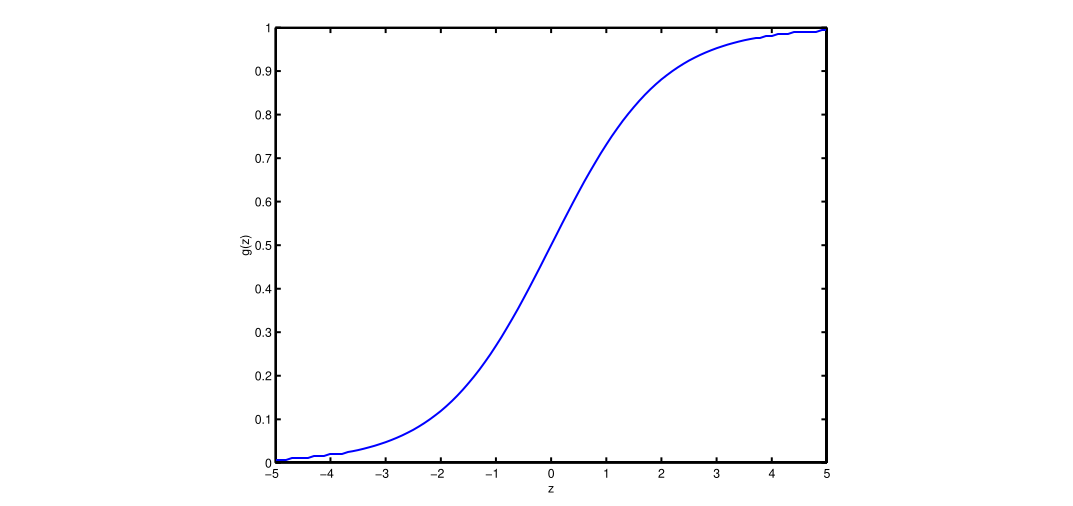
\includegraphics[width=10cm]{1}\\
\end{center}
See that $g(z)$ tends toward 1 as $z\to\infty$, and to 0 as $z\to-\infty$. Also see
that it is always bounded between 0 and 1. As before we keep the convention of $x_0=1$, so that
$\theta^Tx=\theta_0+\sum^d_{j=1}\theta_jx_j$.
\end{figure}\\
(next page)
\newpage
\noindent\textbf{Derivative of the Sigmoid function}\\
Defining $g$ as the sigmoid function, we note its derivative:
\begin{align*}
g'(z)&=\frac{d}{dz}\frac{1}{1+e^{-z}}\\
&=\frac{1}{(1+e^{-z})^2}(e^{-z})\\
&=\frac{1}{(1+e^{-z})}\cdot\left(1-\frac{1}{(1+e^{-z})}\right)\\
&=g(z)(1-g(z))
\end{align*}
\textbf{Probabalistic assumptions and maximum likelihood}\\
Here we fit our model via maximum likelihood. For that
we need to make a set of probabalistic assumptions; let us assume that
\begin{align*}
P(y=1|x;\theta)&=h_\theta(x)\\
P(y=0|x;\theta)&=1-h_\theta(x)
\end{align*}
We can write down the probability function for a \textit{single} trial as
\begin{equation*}
p(y|x;\theta)=(h_\theta(x))^y(1-h_\theta(x))^{1-y}
\end{equation*}
Assuming the $n$ training examples were generated independently, we write down the likelihood as
\begin{align*}
L(\theta)&=p(\bm{y}|X;\theta)\\
&=\prod^n_{i=1}p(y^{(i)}|x^{(i)};\theta)\\
&=\prod^n_{i=1}(h_\theta(x^{(i)}))^{y^{(i)}}(1-h_\theta(x^{(i)}))^{1-y^{(i)}}
\end{align*}
To make things easier we maximise the log likelihood:
\begin{equation*}
\ell(\theta)=\log L(\theta)=\sum^n_{i=1}\left[
y^{(i)}\log(h(x^{(i)})+(1-y^{(i)})\log(1-h(x^{(i)}))\right]
\end{equation*}
Here we have the choice of batch or stochastic gradient \textit{ascent}, since we are \textit{maximising}
the likelihood (same as if we maximised log likelihood).\\
(next page)
\newpage
\noindent\textbf{Stochastic gradient ascent rule}\\
Since we are trying to \textit{maximise}, our update rule looks like
\begin{equation*}
\theta:=\theta+\alpha\nabla_\theta\ell(\theta)
\end{equation*}
(Note the positive rather than the negative sign in the update). Here we consider \textit{stochastic} gradient
ascent, so we look at \textit{one} training example and take the derivative
to get the rule (if we took the derivative of the log likelihood we found earlier that would be batch
gradient ascent):
\begin{align*}
\frac{\partial}{\partial\theta_j}\ell(\theta)
&=\left(y\frac{1}{g(\theta^Tx)}-(1-y)\frac{1}{1-g(\theta^Tx)}\right)\frac{\partial}{\partial\theta_j}g(\theta^Tx)\\
\text{(chain rule)}\quad&=\left(y\frac{1}{g(\theta^Tx)}-(1-y)\frac{1}{1-g(\theta^Tx)}\right)
g(\theta^Tx)(1-g(\theta^Tx))\frac{\partial}{\partial\theta_j}\theta^Tx\\
&=(y(1-g(\theta^Tx))-(1-y)g(\theta^Tx))x_j\\
&=(y-g(\theta^Tx))x_j=(y-h_\theta(x))x_j
\end{align*}
In the second equality we used the chain rule and the derivative of $g$ as derived earlier. We now
have the stochastic gradient ascent rule:
\begin{equation*}
\theta_j:=\theta_j+\alpha(y^{(i)}-h_\theta(x^{(i)}))x^{(i)}_j
\end{equation*}
This appears similar to the LMS update rule, but this time our hypothesis $h$ is different.\\
\vspace{1mm}\\
\textbf{Link to logistic loss}\\
Our rule can be viewed as a loss function by defining
$\ell_\text{logistic}:\mathbb{R}\times\{0,1\}\to\mathbb{R}_{\geq0}$
to be the \textit{logistic loss}:
\begin{equation*}
\ell_\text{logistic}(t,y)\triangleq y\log(1+\exp(-t))+
(1-y)\log(1+\exp(t))
\end{equation*}
One can verify by plugging in $h_\theta(x)=1/(1+e^{-\theta^Tx})$ (which is our hypothesis here)
that the \textit{negative} log likelihood can be rewritten as
\begin{equation*}
-\ell(\theta)=\ell_\text{logistic}(\theta^Tx,y)
\end{equation*}
(maximising the likelihood is the same as minimising the \textit{negative} likelihood)
\newpage

\subsection{Logistic regression and Perceptrons}
Consider modifying the logistic regression method to `force' it to output values that are
either 0 or 1 exactly. This can be done by changing the definition of $g$ to be the threshold function:
\begin{equation*}
g(z)=\begin{cases}
1&\text{if }z\geq0\\
0&\text{if }z<0
\end{cases}
\end{equation*}
If we then let $h_\theta(x)=g(\theta^Tx)$ as before but using this modified definition of $g$, with the
same update rule:
\begin{equation*}
\theta_j:=\theta_j+\alpha(y^{(i)}-h_\theta(x^{(i)}))x^{(i)}_j
\end{equation*}
then we have the \textit{perceptron learning algorithm}.
Note that the perceptron is a very type of algorithm to logistic regression or least squares regression. 
\newpage

\subsection{Multi-class softmax classification}
\textbf{Multinomial distribution}\\
Consider a classification problem where the response variable $y$ takes on any one of $k$ discrete values, so
$y\in\{1,2,\ldots,k\}$. We can model this as distributed according to a \textit{multinomial distribution}.\\
\vspace{1mm}\\
The idea of a multinomial distribution is just a generalisation of the binomial---think instead of 
2 possible outcomes per trial for n trials (binomial), we have k possible outcomes per trial for n trials (multinomial).\\
\vspace{1mm}\\
In this case, $p(y|x;\theta)$ is a distribution over $k$ possible discrete outcomes (multinomial). 
A multinomial distribution involves $k$ numbers $\phi_1,\ldots,\phi_k$ specifying
the probability of each outcome. Naturally this also means they must satisfy
\begin{equation*}
\sum^k_{i=1}\phi_i=1
\end{equation*}
\textbf{Softmax}\\
We introduce $k$ groups of parameters $\theta_1,\ldots,\theta_k$ (for $k$ possible outcomes), each of them being a
vector in $\mathbb{R}^d$ (corresponding to number of features). Intuitively, we would like to use
$\theta_1^Tx,\ldots,\theta_k^Tx$ to represent $\phi_1,\ldots,\phi_k$ which correspond to the probabilities:
\begin{equation*}
\phi_i=P(y=i|x;\theta)
\end{equation*}
However, this won't work since the all the $\theta_j^Tx$ don't sum to 1, and they don't necessarily individually
fall within $[0,1]$ anyway.\\
\vspace{1mm}\\
Thus, we consider the \textit{softmax} function to turn $(\theta_1^Tx,\cdots,\theta_k^Tx)$ into a probability 
vector with nonnegative entries that sum to 1. We define
softmax :$\mathbb{R}^k\to\mathbb{R}^k$ as
\begin{equation*}
\text{softmax}(t_1,\ldots,t_k)=\begin{bmatrix}
\frac{\exp(t_1)}{\sum^k_{j=1}\exp(t_j)}\\\vdots\\
\frac{\exp(t_k)}{\sum^k_{j=1}\exp(t_j)}\end{bmatrix}
\end{equation*}
The inputs $t$ are often called \textit{logits}. See that the entries of the output are always
nonnegative and sum to 1.\\
(next page)
\newpage
\noindent\textbf{Softmax (cont.)}\\
Let $(t_1,\ldots,t_k)=(\theta_1^Tx,\cdots,\theta_k^Tx)$.
We apply the softmax function to $(t_1,\ldots,t_k)$ and use the output as probabilities
$P(y=1|x;\theta),\ldots,P(y=k|x;\theta)$:
\begin{equation*}
\begin{bmatrix}P(y=1|x;\theta)\\\vdots\\P(y=k|x;\theta)
\end{bmatrix}=\text{softmax}(t_1,\cdots,t_k)=
\begin{bmatrix}
\frac{\exp(t_1)}{\sum^k_{j=1}\exp(t_j)}\\\vdots\\
\frac{\exp(t_k)}{\sum^k_{j=1}\exp(t_j)}\end{bmatrix}
\end{equation*}
Essentially we let
\begin{equation*}
P(y=i|x;\theta)=\phi_i=\frac{\exp(t_i)}{\sum^k_{j=1}\exp(t_j)}=\frac{\exp(\theta_i^Tx)}{\sum^k_{j=1}
\exp(\theta_j^Tx)}
\end{equation*}
\textbf{Likelihood and cross-entropy}\\
Considering a \textit{single example}, we can write down
the \textit{negative} log-likelihood as
\begin{equation*}
-\log p(y|x,\theta)=-\log\left(\frac{\exp(t_y)}{\sum^k_{j=1}\exp(t_j)}\right)
=-\log\left(\frac{\exp(\theta_y^Tx)}{\sum^k_{j=1}\exp(\theta_j^Tx)}\right)
\end{equation*}
See that we can write down the negative log-likelihood of \textit{all the training data} as
\begin{equation*}
\ell(\theta)=\sum^n_{i=1}-\log\left(\frac{\exp(\theta_{y^{(i)}}^Tx^{(i)})}{\sum^k_{j=1}
\exp(\theta_j^Tx^{(i)})}\right)
\end{equation*}
Defining the \textit{Cross-entropy loss} $\ell_{\text{ce}}:\mathbb{R}^k\times\{1,\ldots,k\}
\to\mathbb{R}_{\geq0}$ (its just the negative log likelihood for one trial):
\begin{equation*}
\ell_{\text{ce}}((t_1,\ldots,t_k),y)=-\log\left(\frac{\exp(t_y)}{\sum^k_{j=1}\exp(t_j)}\right)
\end{equation*}
With that we can rewrite the negative log-likelihood of all the training data as
\begin{equation*}
\ell(\theta)=\sum^n_{i=1}\ell_{\text{ce}}((\theta_1^Tx^{(i)},\ldots,\theta_k^Tx^{(i)}),y^{(i)})
\end{equation*}
(We want to `tune' all the $\theta$ to maximise the likelihood/minimise the negative likelihood
of the features $x^{(i)}$ `predicting' $y^{(i)}$.)\\
(next page)
\newpage
\noindent\textbf{Minimising the cross-entropy}\\
We had the cross-entropy
\begin{equation*}
\ell_{\text{ce}}((t_1,\ldots,t_k),y)=-\log\left(\frac{\exp(t_y)}{\sum^k_{j=1}\exp(t_j)}\right)
\end{equation*}
The cross-entropy has a simple gradient. Letting 
$t=(t_1,\ldots,t_k)$ and recalling $\phi_i=\frac{\exp(t_i)}{\sum^k_{j=1}\exp(t_j)}$, we can derive
\begin{equation*}
\frac{\partial\ell_{\text{ce}}(t,y)}{\partial t_i}=\phi_i-1\{y=i\}
\end{equation*}
In vectorised notation we have the following form
\begin{equation*}
\frac{\partial\ell_{\text{ce}}(t,y)}{\partial t}=\phi-e_y
\end{equation*}
where $e_s\in\mathbb{R}^k$ is the $s$-th natural basis vector (where the $s$-th entry is 1 and all other entries
are zeros).\\
\vspace{1mm}\\
\textbf{With respect to $\theta$}\\
We want the gradient with respect to $\theta$; using the chain rule we have (for single example)
\begin{equation*}
\frac{\partial\ell_{\text{ce}}((\theta_1^Tx,\ldots,\theta_k^Tx),y)}{\partial\theta_i}
=\frac{\partial\ell(t,y)}{\partial t_i}\cdot\frac{\partial t_i}{\partial\theta_i}=(\phi_i-1\{y=i\})\cdot x
\end{equation*}
We now have the gradient of the loss with respect to $\theta_i$ for the training data as
\begin{equation*}
\frac{\partial\ell(\theta)}{\partial\theta_i}
=\sum^n_{j=1}(\phi_i^{(j)}-1\{y^{(j)}=i\})\cdot x^{(j)}
\end{equation*}
Remember that $\phi_i=\frac{\exp(t_i)}{\sum^k_{j=1}\exp(t_j)}$ denotes the predicted probability \textit{given the training example} and 
$\theta$, and thus its
value changes with each example (hence the superscript).
\newpage

\subsection{Derivation of gradient for cross-entropy loss}
The cross-entropy loss is given by
\begin{equation*}
\ell_{\text{ce}}((t_1,\ldots,t_k),y)=-\log\left(\frac{\exp(t_y)}{\sum^k_{j=1}\exp(t_j)}\right)
\end{equation*}
Letting $t=(t_1,\ldots,t_k)$ and recalling $\phi_i=\frac{\exp(t_i)}{\sum^k_{j=1}\exp(t_j)}$, 
we take the gradient with respect to $t_i$. This falls into two cases:\\
\vspace{1mm}\\
\textbf{First case:} $y=i$\\
Using the chain rule:
\begin{equation*}
\frac{\partial}{\partial t_y}(-\log(\phi_y))=
\frac{\partial}{\partial\phi_y}(-\log(\phi_y))\cdot
\frac{\partial\phi_y}{\partial t_y}=-\frac{1}{\phi_y}\cdot
\frac{\partial\phi_y}{\partial t_y}
\end{equation*}
now product rule:
\begin{align*}
-\frac{1}{\phi_y}\cdot\frac{\partial\phi_y}{\partial t_y}
&=-\frac{1}{\phi_y}\cdot\left(\phi_y+\left(-\frac{(\exp(t_y))^2}{\left(\sum^k_{j=1}\exp(t_j)\right)^2}\right)\right)
\\&=-1+\frac{\sum^k_{j=1}\exp(t_j)}{\exp(t_y)}\cdot\frac{(\exp(t_y))^2}{\left(\sum^k_{j=1}\exp(t_j)\right)^2}\\
&=\frac{\exp(t_y)}{\sum^k_{j=1}\exp(t_j)}-1=\phi_y-1
\end{align*}
\textbf{Second case:} $y\neq i$\\
Same as before
\begin{equation*}
\frac{\partial}{\partial t_{i\neq y}}(-\log(\phi_y))=
\frac{\partial}{\partial\phi_y}(-\log(\phi_y))\cdot
\frac{\partial\phi_y}{\partial t_{i\neq y}}=-\frac{1}{\phi_y}\cdot
\frac{\partial\phi_y}{\partial t_{i\neq y}}
\end{equation*}
but now instead we have
\begin{align*}
-\frac{1}{\phi_y}\cdot\frac{\partial\phi_y}{\partial t_{i\neq y}}&=
\frac{\sum^k_{j=1}\exp(t_j)}{\exp(t_y)}\cdot
\frac{\exp(t_y)\exp(t_{i\neq y})}{\left(\sum^k_{j=1}\exp(t_j)\right)^2}=\phi_{i\neq y}
\end{align*}
\textbf{Compact form}\\
We can therefore write
\begin{equation*}
\frac{\partial\ell_{\text{ce}}(t,y)}{\partial t_i}=\phi_i-1\{y=i\}
\end{equation*}
Where $1\{\cdot\}$ denotes the indicator function.
\newpage

\subsection{}










\end{document}
